% Neurone artificiel (somme pondérée + activation) -> ../neurone.pdf
% Compilation : xelatex -output-directory=.. neurone.tex
\documentclass[tikz,border=4pt]{standalone}
\definecolor{hearcred}{HTML}{FF0000}
\definecolor{hearcgray}{HTML}{6E6E6E}
\begin{document}
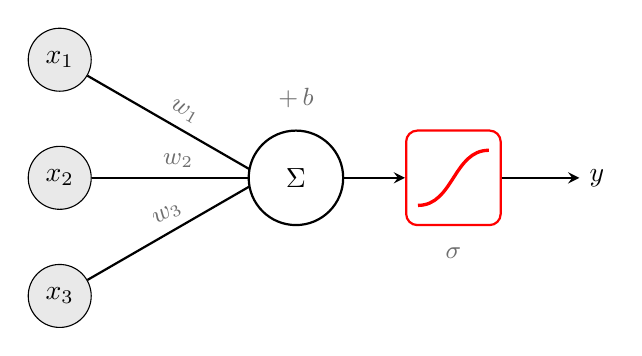
\begin{tikzpicture}[
    font=\sffamily,
    entree/.style={circle, draw=black, fill=hearcgray!15, minimum size=0.8cm},
    fleche/.style={->, >=stealth, line width=0.8pt},
  ]
  \foreach \i/\y in {1/1.5, 2/0, 3/-1.5} {
    \node[entree] (x\i) at (0, \y) {$x_\i$};
    \draw[fleche] (x\i) -- node[above, sloped, font=\small, text=hearcgray] {$w_\i$} (2.6, 0);
  }
  \node[circle, draw=black, line width=0.8pt, minimum size=1.2cm, fill=white] (somme) at (3, 0) {$\Sigma$};
  \node[draw=hearcred, line width=0.8pt, rounded corners, minimum size=1.2cm] (act) at (5, 0) {};
  \draw[hearcred, line width=1.2pt] (4.55, -0.35) .. controls (5.0, -0.35) and (5.0, 0.35) .. (5.45, 0.35);
  \draw[fleche] (somme) -- (act);
  \draw[fleche] (act) -- (6.6, 0) node[right] {$y$};
  \node[above=0.15cm, font=\small, text=hearcgray] at (somme.north) {$+\,b$};
  \node[below=0.15cm, font=\small, text=hearcgray] at (act.south) {$\sigma$};
\end{tikzpicture}
\end{document}
